\documentclass{anstrans}
%%%%%%%%%%%%%%%%%%%%%%%%%%%%%%%%%%%
\title{A nuclear energy-based approach for dealing with the duck curve}
\author{Roberto E. Fairhurst Agosta}

\institute{
University of Illinois at Urbana-Champaign, Dept. of Nuclear, Plasma, and Radiological Engineering\\
ref3@illinois.edu
}

%%%% packages and definitions (optional)
\usepackage{graphicx} % allows inclusion of graphics
\usepackage{booktabs} % nice rules (thick lines) for tables
\usepackage{microtype} % improves typography for PDF
\usepackage{xspace}
\usepackage{tabularx}
\usepackage{floatrow}
\usepackage{subcaption}
\usepackage{enumitem}
\usepackage{placeins}
\usepackage{amsmath}
\usepackage[acronym,toc]{glossaries}
\newacronym[longplural={metric tons of heavy metal}]{MTHM}{MTHM}{metric ton of heavy metal}
\newacronym{ABM}{ABM}{agent-based modeling}
\newacronym{ANL}{ANL}{Argonne National Laboratory}
\newacronym{ARFC}{ARFC}{Advanced Reactors and Fuel Cycles}
\newacronym{BOL}{BOL}{Beginning-of-Life}

\newacronym{BSD}{BSD}{Berkeley Software Distribution}
\newacronym{CO2}{$CO_2$}{carbon dioxide}
\newacronym{CAFCA}{CAFCA}{ Code for Advanced Fuel Cycles Assessment }
\newacronym{CASL}{CASL}{Consortium for Advanced Simulation of Light Water Reactors}
\newacronym{CDTN}{CDTN}{Centro de Desenvolvimento da Tecnologia Nuclear}
\newacronym{CEA}{CEA}{Commissariat \`a l'\'Energie Atomique et aux \'Energies Alternatives}
\newacronym{CI}{CI}{continuous integration}
\newacronym{CNEC}{CNEC}{Consortium for Nonproliferation Enabling Capabilities}
\newacronym{CNEN}{CNEN}{Comiss\~{a}o Nacional de Energia Nuclear}
\newacronym{CNERG}{CNERG}{Computational Nuclear Engineering Research Group}
\newacronym{COSI}{COSI}{Commelini-Sicard}
\newacronym{COTS}{COTS}{commercial, off-the-shelf}
\newacronym{CSNF}{CSNF}{commercial spent nuclear fuel}
\newacronym{CTAH}{CTAHs}{Coiled Tube Air Heaters}
\newacronym{CUBIT}{CUBIT}{CUBIT Geometry and Mesh Generation Toolkit}
\newacronym{CURIE}{CURIE}{Centralized Used Fuel Resource for Information Exchange}
\newacronym{DAG}{DAG}{directed acyclic graph}
\newacronym{DANESS}{DANESS}{Dynamic Analysis of Nuclear Energy System Strategies}
\newacronym{DBE}{DBE}{Design Basis Event}
\newacronym{DESAE}{DESAE}{Dynamic Analysis of Nuclear Energy Systems Strategies}
\newacronym{DHS}{DHS}{Department of Homeland Security}
\newacronym{DOE}{DOE}{Department of Energy}
\newacronym{DRACS}{DRACS}{Direct Reactor Auxiliary Cooling System}
\newacronym{DRE}{DRE}{dynamic resource exchange}
\newacronym{DSNF}{DSNF}{DOE spent nuclear fuel}
\newacronym{DYMOND}{DYMOND}{Dynamic Model of Nuclear Development }
\newacronym{EBS}{EBS}{Engineered Barrier System}
\newacronym{EDZ}{EDZ}{Excavation Disturbed Zone}
\newacronym{EIA}{EIA}{U.S. Energy Information Administration}
\newacronym{EPA}{EPA}{Environmental Protection Agency}
\newacronym{EP}{EP}{Engineering Physics}
\newacronym{FCO}{FCO}{Fuel Cycle Options}
\newacronym{FCT}{FCT}{Fuel Cycle Technology}
\newacronym{FCWMD}{FCWMD}{Fuel Cycle and Waste Management Division}
\newacronym{FEHM}{FEHM}{Finite Element Heat and Mass Transfer}
\newacronym{FEPs}{FEPs}{Features, Events, and Processes}
\newacronym{FHR}{FHR}{Fluoride-Salt-Cooled High-Temperature Reactor}
\newacronym{FLiBe}{FLiBe}{Fluoride-Lithium-Beryllium}
\newacronym{FCEV}{FCEV}{fuel cell electric vehicles}
\newacronym{GGE}{GGE}{gasoline gallon equivalent}
\newacronym{GCAM}{GCAM}{Global Change Assessment Model}
\newacronym{DGE}{DGE}{diesel gallon equivalent}
\newacronym{GDSE}{GDSE}{Generic Disposal System Environment}
\newacronym{GDSM}{GDSM}{Generic Disposal System Model}
\newacronym{GENIUSv1}{GENIUSv1}{Global Evaluation of Nuclear Infrastructure Utilization Scenarios, Version 1}
\newacronym{GENIUSv2}{GENIUSv2}{Global Evaluation of Nuclear Infrastructure Utilization Scenarios, Version 2}
\newacronym{GENIUS}{GENIUS}{Global Evaluation of Nuclear Infrastructure Utilization Scenarios}
\newacronym{GPAM}{GPAM}{Generic Performance Assessment Model}
\newacronym{GHG}{GHG}{greenhouse gas}
\newacronym{GRSAC}{GRSAC}{Graphite Reactor Severe Accident Code}
\newacronym{GUI}{GUI}{graphical user interface}
\newacronym{HLW}{HLW}{high level waste}
\newacronym{HPC}{HPC}{high-performance computing}
\newacronym{HTC}{HTC}{high-throughput computing}
\newacronym{HTR}{HTR}{high temperature reactor}
\newacronym{IAEA}{IAEA}{International Atomic Energy Agency}
\newacronym{ICAP}{ICAP}{Illinois Climate Action Plan}
\newacronym{IEMA}{IEMA}{Illinois Emergency Mangament Agency}

\newacronym{INL}{INL}{Idaho National Laboratory}
\newacronym{LANL}{LANL}{Los Alamos National Laboratory}
\newacronym{LLNL}{LLNL}{Lawrence Livermore National Laboratory}

\newacronym{LWR}{LWR}{Light Water Reactor}
\newacronym{MARKAL}{MARKAL}{MARKet and ALlocation}
\newacronym{MA}{MA}{minor actinide}
\newacronym{MCNP}{MCNP}{Monte Carlo N-Particle code}
\newacronym{MILP}{MILP}{mixed-integer linear program}

\newacronym{MOAB}{MOAB}{Mesh-Oriented datABase}
\newacronym{MOOSE}{MOOSE}{Multiphysics Object-Oriented Simulation Environment}
\newacronym{MOX}{MOX}{mixed oxide}
\newacronym{MSBR}{MSBR}{Molten Salt Breeder Reactor}
\newacronym{MSRE}{MSRE}{Molten Salt Reactor Experiment}
\newacronym{MSR}{MSR}{Molten Salt Reactor}
\newacronym{MTD}{MTD}{Champaign-Urbana Mass Transit District}

\newacronym{NCSA}{NCSA}{National Center for Supercomputing Applications}
\newacronym{NEAMS}{NEAMS}{Nuclear Engineering Advanced Modeling and Simulation}
\newacronym{NEUP}{NEUP}{Nuclear Energy University Programs}
\newacronym{NFCSim}{NFCSim}{Nuclear Fuel Cycle Simulator}
\newacronym{NFC}{NFC}{Nuclear Fuel Cycle}
\newacronym{NGNP}{NGNP}{Next Generation Nuclear Plant}
\newacronym{NMWPC}{NMWPC}{Nuclear MW Per Capita}
\newacronym{NNSA}{NNSA}{National Nuclear Security Administration}
\newacronym{NPRE}{NPRE}{Department of Nuclear, Plasma, and Radiological Engineering}
\newacronym{NQA1}{NQA-1}{Nuclear Quality Assurance - 1}
\newacronym{NRC}{NRC}{Nuclear Regulatory Commission}
\newacronym{NSF}{NSF}{National Science Foundation}
\newacronym{NSSC}{NSSC}{Nuclear Science and Security Consortium}
\newacronym{NUWASTE}{NUWASTE}{Nuclear Waste Assessment System for Technical Evaluation}
\newacronym{NWF}{NWF}{Nuclear Waste Fund}
\newacronym{NWTRB}{NWTRB}{Nuclear Waste Technical Review Board}
\newacronym{OCRWM}{OCRWM}{Office of Civilian Radioactive Waste Management}
\newacronym{ORION}{ORION}{ORION}
\newacronym{ORNL}{ORNL}{Oak Ridge National Laboratory}
\newacronym{PARCS}{PARCS}{Purdue Advanced Reactor Core Simulator}
\newacronym{PBAHTR}{PB-AHTR}{Pebble Bed Advanced High Temperature Reactor}
\newacronym{PBFHR}{PB-FHR}{Pebble-Bed Fluoride-Salt-Cooled High-Temperature Reactor}
\newacronym{PEI}{PEI}{Peak Environmental Impact}
\newacronym{PH}{PRONGHORN}{PRONGHORN}
\newacronym{PI}{PI}{Principal Investigator}
\newacronym{PNNL}{PNNL}{Pacific Northwest National Laboratory}
\newacronym{PRIS}{PRIS}{Power Reactor Information System}
\newacronym{PRKE}{PRKE}{Point Reactor Kinetics Equations}
\newacronym{PSPG}{PSPG}{Pressure-Stabilizing/Petrov-Galerkin}
\newacronym{PWAR}{PWAR}{Pratt and Whitney Aircraft Reactor}
\newacronym{PWR}{PWR}{Pressurized Water Reactor}
\newacronym{PyNE}{PyNE}{Python toolkit for Nuclear Engineering}
\newacronym{PyRK}{PyRK}{Python for Reactor Kinetics}
\newacronym{QA}{QA}{quality assurance}
\newacronym{RDD}{RD\&D}{Research Development and Demonstration}
\newacronym{RD}{R\&D}{Research and Development}
\newacronym{RELAP}{RELAP}{Reactor Excursion and Leak Analysis Program}
\newacronym{RIA}{RIA}{Reactivity Insertion Accident}
\newacronym{RIF}{RIF}{Region-Institution-Facility}
\newacronym{SAM}{SAM}{Simulation and Modeling}
\newacronym{SCF}{SCF}{Software Carpentry Foundation}
\newacronym{SFR}{SFR}{Sodium-Cooled Fast Reactor}
\newacronym{SI}{SI}{sulfur-iodine}
\newacronym{SINDAG}{SINDA{\textbackslash}G}{Systems Improved Numerical Differencing Analyzer $\backslash$ Gaski}
\newacronym{SKB}{SKB}{Svensk K\"{a}rnbr\"{a}nslehantering AB}
\newacronym{SNF}{SNF}{spent nuclear fuel}
\newacronym{SNL}{SNL}{Sandia National Laboratory}
\newacronym{SNM}{SNM}{Special Nuclear Material}
\newacronym{STC}{STC}{specific temperature change}
\newacronym{SUPG}{SUPG}{Streamline-Upwind/Petrov-Galerkin}
\newacronym{SWF}{SWF}{Separations and Waste Forms}
\newacronym{SWU}{SWU}{Separative Work Unit}
\newacronym{SandO}{S\&O}{Signatures and Observables}
\newacronym{THW}{THW}{The Hacker Within}
\newacronym{TRIGA}{TRIGA}{Training Research Isotope General Atomic}
\newacronym{TRISO}{TRISO}{Tristructural Isotropic}
\newacronym{TSM}{TSM}{Total System Model}
\newacronym{TSPA}{TSPA}{Total System Performance Assessment for the Yucca Mountain License Application}
\newacronym{UDB}{UDB}{Unified Database}
\newacronym{UFD}{UFD}{Used Fuel Disposition}
\newacronym{UIUC}{UIUC}{University of Illinois at Urbana-Champaign}
\newacronym{UML}{UML}{Unified Modeling Language}
\newacronym{UNFSTANDARDS}{UNFST\&DARDS}{Used Nuclear Fuel Storage, Transportation \& Disposal Analysis Resource and Data System}
\newacronym{UOX}{UOX}{uranium oxide}
\newacronym{US}{US}{United States}
\newacronym{VISION}{VISION}{the Verifiable Fuel Cycle Simulation Model}
\newacronym{VV}{V\&V}{verification and validation}
\newacronym{NEI}{NEI}{Nuclear Energy Institute}
%\newacronym{<++>}{<++>}{<++>}
%\newacronym{<++>}{<++>}{<++>}

\makeglossaries

\usepackage[printwatermark]{xwatermark}
\usepackage{xcolor}
\usepackage{graphicx}
\usepackage{lipsum}
\usepackage{indentfirst}  % to indent first paragraph

\newcommand{\SN}{S$_N$}
\renewcommand{\vec}[1]{\bm{#1}} %vector is bold italic
\newcommand{\vd}{\bm{\cdot}} % slightly bold vector dot
\newcommand{\grad}{\vec{\nabla}} % gradient
\newcommand{\ud}{\mathop{}\!\mathrm{d}} % upright derivative symbol

\newcolumntype{c}{>{\hsize=.56\hsize}X}
\newcolumntype{b}{>{\hsize=.7\hsize}X}
\newcolumntype{s}{>{\hsize=.74\hsize}X}
\newcolumntype{f}{>{\hsize=.1\hsize}X}
\newcolumntype{a}{>{\hsize=.45\hsize}X}
%\usepackage[pagestyles]{titlesec}
%\titleformat*{\subsection}{\normalfont}
%\titleformat{\section}{\bfseries}{Item \thesection.\ }{0pt}{}

%\newwatermark[allpages,color=gray!50,angle=45,scale=3,xpos=0,ypos=0]{DRAFT}

\begin{document}
%%%%%%%%%%%%%%%%%%%%%%%%%%%%%%%%%%%%%%%%%%%%%%%%%%%%%%%%%%%%%%%%%%%%%%%%%%%%%%%%
\section{Introduction}
\label{intro}

% very intro
Energy is one of the strongest contributors to economic growth.
In the future, economies will continue to grow, populations will do so too, and their energy demand will accompany such growth \cite{burke_impact_2018}.
Meeting these future needs requires the development of clean energy sources as environmental concerns continue to rise.
As seen in Figure \ref{fig:ghg}, electricity generation is one of the economic sectors that produced the most \glspl{GHG} in the \gls{US} in 2017.
As \gls{CO2} is the main component in \glspl{GHG}, decarbonizing electricity generation will allow us to meet the increases in energy demand and address the environmental concerns at the same time.

\begin{figure}[htbp!]
	\centering
	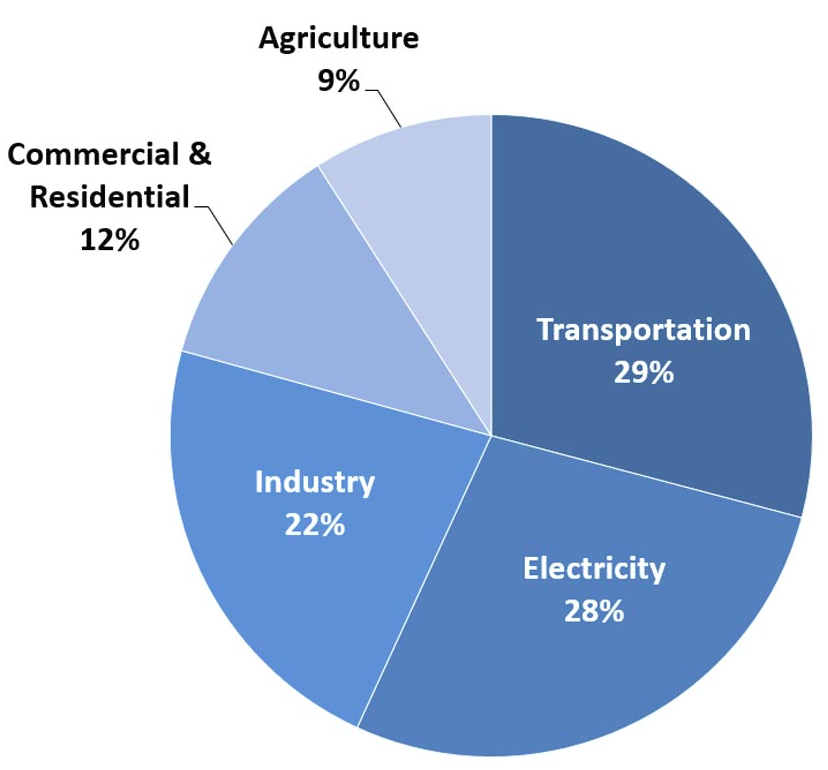
\includegraphics[width=0.6\linewidth]{figures/total-ghg-2019-caption2.png}
	\hfill
	\caption{Total U.S. GHG Emissions by Economic Sector in 2017 \cite{us_epa_sources_2020}.}
	\label{fig:ghg}
\end{figure}

% word on solar energy and the duck curve
To address these concerns, utilities are relying more on intermittent renewable energy resources, such as wind and solar \cite{ming_resource_2019}.
However, high solar adoption creates a challenge. The need for electricity generators to quickly ramp up increases when the sun sets and the contribution from the \gls{PV} falls \cite{us_department_of_energy_confronting_2017}.
The "duct chart" (or duck curve) depicts this phenomenon, Figure \ref{fig:duck}.
The California ISO developed the duck curve to illustrate the difference between forecast load and expected electricity production from solar \cite{bouillon_prepared_2014}.
Moreover, the duck curve reveals another issue. Over-generation may occur during the middle of the day and high-levels of non-dispatchable generation may exacerbate the situation \cite{bouillon_prepared_2014}.

\begin{figure}[htbp!]
	\centering
	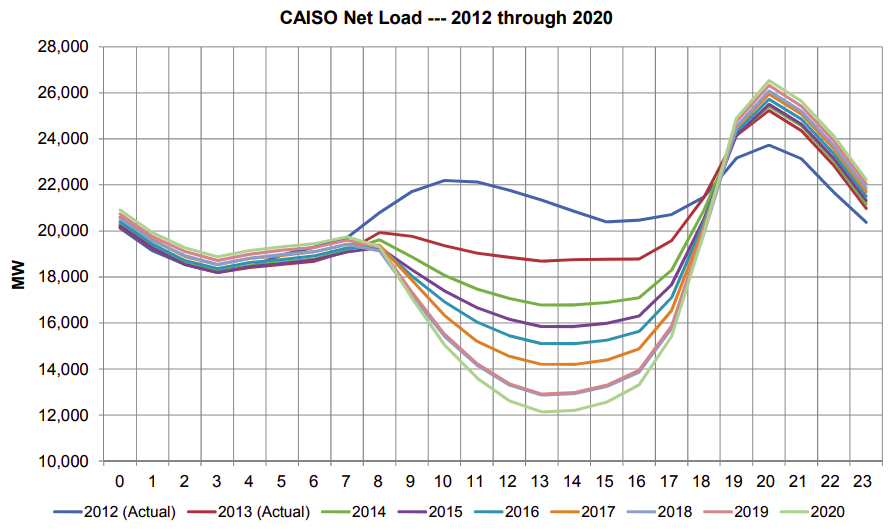
\includegraphics[width=1.0\linewidth]{figures/caiso-duck.png}
	\hfill
	\caption{The duck curve \cite{bouillon_prepared_2014}.}
	\label{fig:duck}
\end{figure}

% solutions to the duck curve
The simplest solution to a demand ramp up is to increase dispatchable generation, such as natural gas and coal \cite{bouillon_prepared_2014}, and decrease non-dispatchable generation, such as geothermal, nuclear, and hydro.
Nonetheless, an approach like this is not consistent with the goal of reducing carbon emissions.
Hence, our focus drifts to other potential low-carbon solutions, like nuclear generation and electricity storage by means of hydrogen production.

As mentioned earlier, the duck curve reveals a risk of over-generation due to high levels of non-dispatchable capacity.
The solution proposed in this article is to use the over-generated energy to produce hydrogen.
The final application of hydrogen could be either supply the transportation sector, or use it to produce electricity during the peak demand in the evening.
While the first solution will reduce the carbon emissions of the transportation sector, the second one will decrease the need for dispatchable sources and, consequently, reduce the carbon emissions of the electricity generation sector.

This article intends to answer the following question: Is the duck curve likely to occur in the \gls{US} grid?
Then, the focus of the analysis narrows down to the \gls{UIUC} grid and studies the impact of producing hydrogen with a nuclear reactor.
The following section briefly introduces two hydrogen production methods and their energy requirements.

\section{Hydrogen production}
\label{section:hydroprod}

This section presents the electrolysis process as a method to couple the production of hydrogen to a nuclear reactor.
Water electrolysis converts electric and thermal energy into chemical energy stored in hydrogen \cite{hi2h2_highly_2007}.
The process enthalpy change $\Delta H$ determines the required energy for the electrolysis reaction to take place.
Part of the energy corresponds to electric energy $\Delta G$ and the rest of it to thermal energy $T \cdot \Delta S$, Figure \ref{fig:electro}.
This gives the relation
\begin{equation}
\Delta H = \Delta G + T \Delta S.
\end{equation}

In liquid water electrolysis or \gls{LTE}, electricity generates the thermal energy.
In steam electrolysis or \gls{HTE}, a high temperature heat source is necessary to provide the thermal energy.
The latter has the advantage that $\Delta G$ decreases with increasing temperature, Figure \ref{fig:electro}.
Since heat-engine-based electrical work is limited to a production thermal efficiency of 50$\%$ or less, decreasing the electricity requirement results in higher overall production efficiencies \cite{j_e_obrien_high_2010}.

\begin{figure}[htbp!]
	\centering
	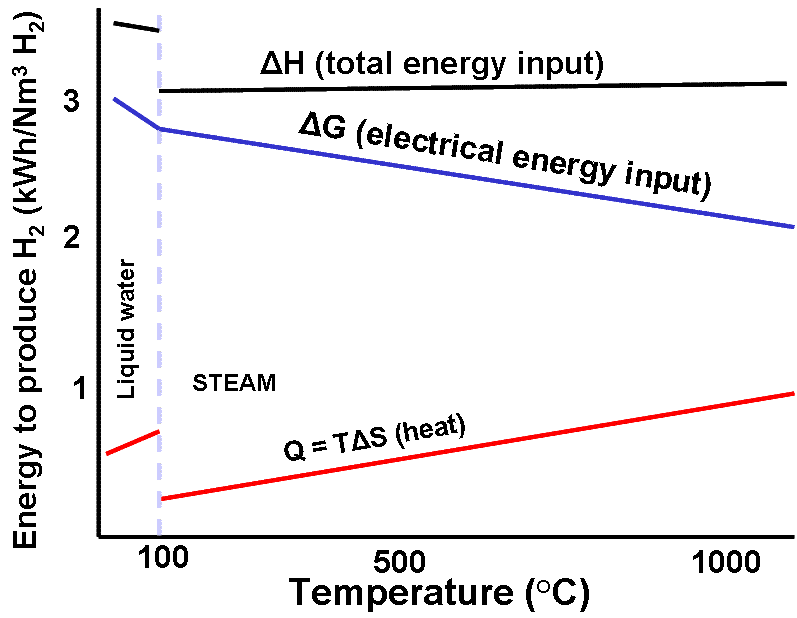
\includegraphics[width=0.7\linewidth]{figures/ele-heat_curve.png}
	\hfill
	\caption{Energy consumption of an ideal electrolysis process \cite{hi2h2_highly_2007}.}
	\label{fig:electro}
\end{figure}

In this analysis, the energy source (both electric and thermal) is a nuclear reactor with co-generation capabilities.
The nuclear reactor supplies the grid with electricity ($P_E$) while providing a hydrogen plant with electricity ($P_{EH2}$) and thermal energy ($P_{TH2}$) Figure \ref{fig:h2diag}.
$\beta$ and $\gamma$ determine the distribution of the reactor thermal power $P_{th}$ into $P_E$, $P_{EH2}$, and $P_{TH2}$.
$\eta$ is the thermal-to-electric energy conversion ratio.
This gives the following relations

\begin{equation}
\begin{split}
P_{E} &= \eta \beta P_{th}
\\
P_{EH2} &= \eta \gamma (1-\beta) P_{th}
\\
P_{TH2} &= (1-\gamma) (1-\beta) P_{th}
\\
\gamma &= \frac{P_{EH2} / \eta}{P_{EH2} / \eta + P_{TH2}}
\\
\beta &= \frac{P_{E} / \eta}{P_{E} / \eta + P_{TH2}/(1-\gamma)}.
\end{split}
\label{eq:hydro}
\end{equation}

With eq. \ref{eq:hydro} we calculate the energy requirements for \gls{LTE} (eq. \ref{eq:hydro-lte}) and \gls{HTE} (eq. \ref{eq:hydro-hte}), respectively. $m_{H_2}$ is the mass of hydrogen manufactured. Note that in \gls{LTE}, electricity provides $T \cdot \Delta S$, making $\gamma$ equal to 1 and $P_{TH2}$ equal to 0.

\begin{equation}
m_{H_2} (\Delta G + T\Delta S) = P_{EH2} = \eta (1-\beta) P_{th}
\label{eq:hydro-lte}
\end{equation}

\begin{equation}
\begin{split}
m_{H_2} \Delta G &= P_{EH2} = \eta \gamma (1-\beta) P_{th}
\\
m_{H_2} T\Delta S &= P_{TH2} = (1-\gamma) (1-\beta) P_{th}
\end{split}
\label{eq:hydro-hte}
\end{equation}

\begin{figure}[htbp!]
	\centering
	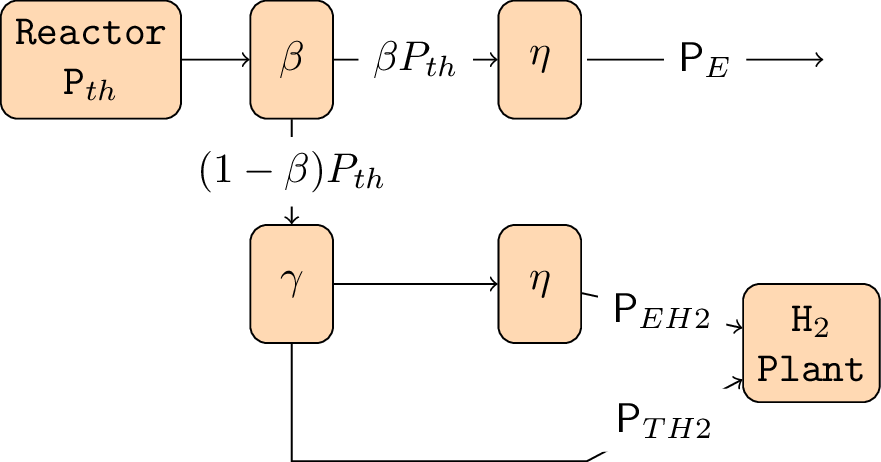
\includegraphics[width=1.0\linewidth]{figures/hte-figure0.png}
	\hfill
	\caption{Diagram of a nuclear power plant connected to the grid and coupled to a hydrogen plant.}
	\label{fig:h2diag}
\end{figure}

\section{Methodology}
\label{method}

Performing a linear regression on data of the total electricity generated in the US by year \cite{us_energy_information_administration_electric_2020} we predict the total electricity generation in the \gls{US} for 2050, Figure \ref{fig:us-pred1}.
Using the same method, we estimate the solar electricity generation in the \gls{US} for 2050, Figure \ref{fig:us-pred2}.

% % Word on the US yearly data
\begin{figure}[H]
	\centering
	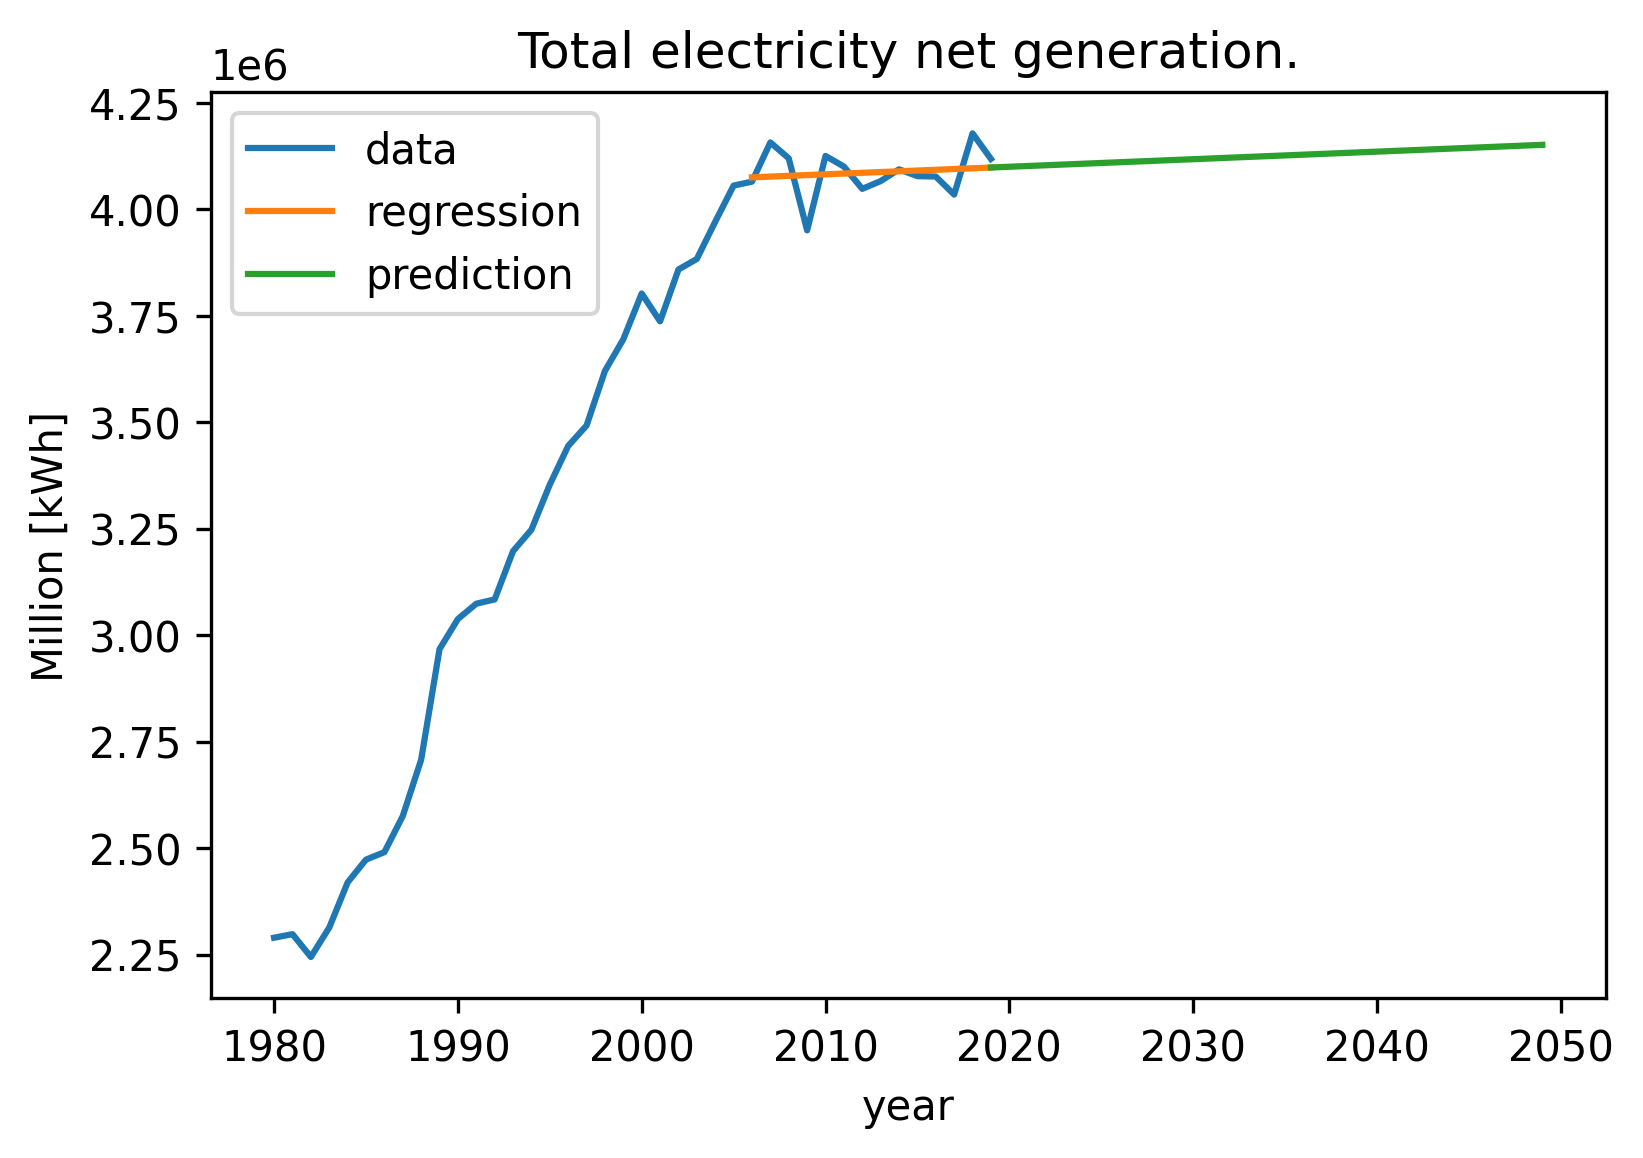
\includegraphics[width=1.0\linewidth]{figures/us-prediction1.png}
	\hfill
	\caption{Prediction on the total electricity generation in the \gls{US} for 2050.}
	\label{fig:us-pred1}
\end{figure}

\begin{figure}[H]
	\centering
	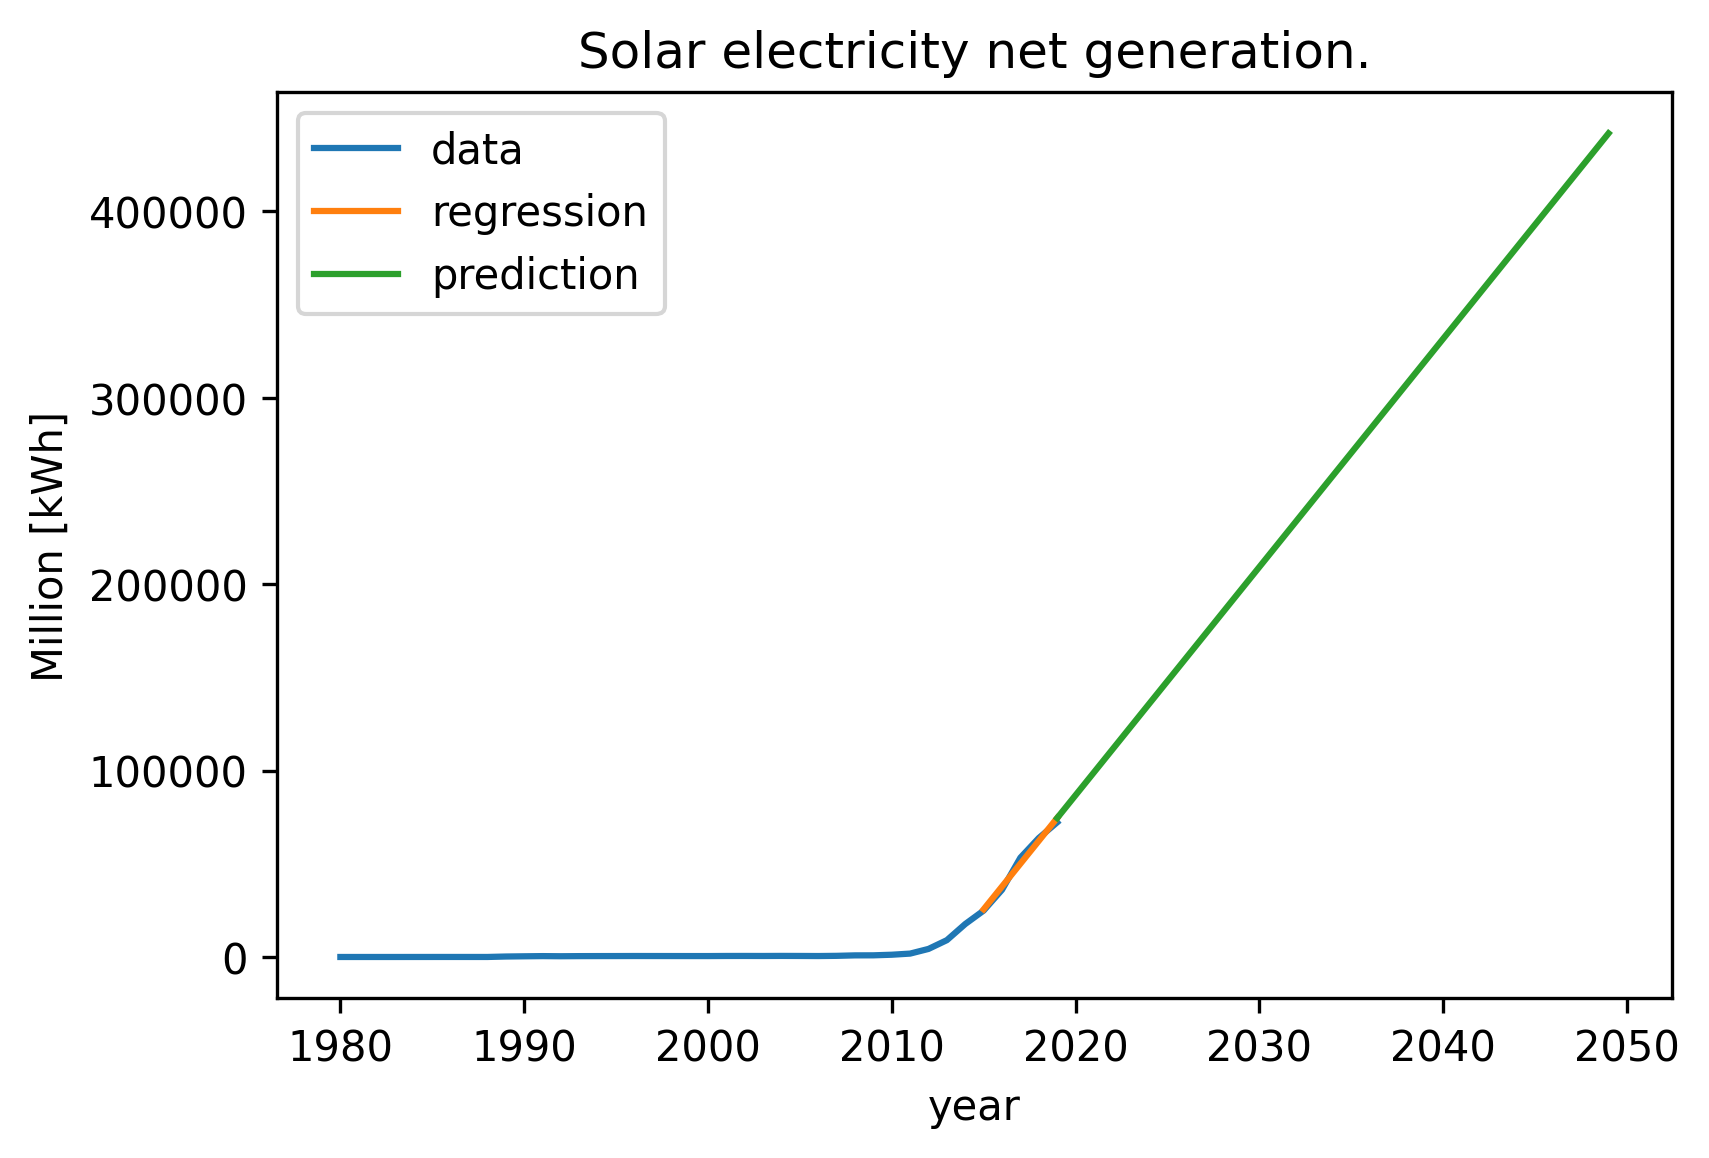
\includegraphics[width=1.0\linewidth]{figures/us-prediction2.png}
	\hfill
	\caption{Prediction on the solar electricity generation in the \gls{US} for 2050.}
	\label{fig:us-pred2}
\end{figure}

The predictions allow us to determine the growth rate of the total ($GR_{T}$) and solar ($GR_{S}$) electricity generation, eq. \ref{GR}. Where $T_i$ and $S_i$ correspond to the total and solar electricity generation in year $i$, respectively. $N$ is the number of years that we are looking into the future.

\begin{equation}
\begin{split}
GR_{T} &= \frac{T_{2050}-T_{2019}} {T_{2019} \cdot N }
\\
GR_{S} &= \frac{S_{2050}-S_{2019}} {S_{2019} \cdot N }
\end{split}
\label{GR}
\end{equation}

To predict the demand by hour we need to choose a day first.
We focus on the spring, when the solar production is higher, as it is sunny, but the total demand is low since people are not using electricity for air conditioning or heating \cite{us_department_of_energy_confronting_2017}.
Then, we apply the growth rate to the electricity generated by hour in 2019 and we obtain a prediction on the demand by hour in 2050.
The demand hourly data is available at \cite{eia_united_2020}.

Once, we have carried out the previous calculations, we repeat the process focusing on the \gls{UIUC} grid.
We apply the growth rate calculated for the \gls{US} on the \gls{UIUC} campus electricity demand.
We choose to use the \gls{US} growth rate as the solar generation data that we count with is scarce, as the solar farm at \gls{UIUC} is relatively new \cite{illinois_facilities_and_services_solar_2020}.

With the demand already predicted, the next step is to calculate the over-generated electricity. For that, we arbitrarily choose a reactor power $P_e$.
We consider that the reactor operates at its maximum capacity at all times. Which makes $P_E = P_e$.
Note that $P_e$ has power units while $P_E$ has energy units.
In our study, the time steps are hours, so their values differ by the constant $1h$.
From now on, we will refer to the demand of electricity produced by sources other than solar as just demand.
Once the demand, $D_i$ becomes smaller than $P_E$, $P_E$ becomes equal to $D_i$, eq. \ref{eq:excess1}.
This makes $P_E < P_e$, and leaves an excess of thermal energy $E_i$.
Finally, we can calculate the amount of hydrogen produced using eq. \ref{eq:hydro}.

\begin{equation}
\begin{split}
P_E &= D_i
\\
\frac{P_E}{P_e} &= \frac{\eta \beta P_{th}}{\eta P_{th}} = \beta
\\
E_i &= (1-\beta) P_{th}
\end{split}
\label{eq:excess1}
\end{equation}

The last step in our analysis is to calculate the reduction of the peak demand by using the hydrogen to produce electricity.
The energy produced by the hydrogen is $285 kJ/mol$, which is equal to $40 kWh/kg$ \cite{ursua_hydrogen_2012}.
However, a fuel cell system can use up to a 60$\%$ of that energy \cite{doe_energy_efficiency_and_renewable_energy_fuel_2015}.
With eq. \ref{eq:hydro}, \ref{eq:hydro-lte}, \ref{eq:hydro-hte}, and \ref{eq:excess1} we compute the mass of hydrogen produced at every hour $m_{H_2i}$.
The total hydrogen mass is $TH$.
The total electricity produced with the hydrogen is $E$, eq. \ref{eq:elect}.

\begin{equation}
\begin{split}
TH &= \sum_i m_{H_{2i}}
\\
E &= 0.6 \times 40 kWh/kg \times TH.
\end{split}
\label{eq:elect}
\end{equation}

The only thing remaining is to to reduce the peak demand by distributing $E$ over the range of hours when the demand is the largest. This produces a new peak $NP$. This new peak is constant during the number of hours we use the hydrogen $T_{H2}$. Eq. \ref{eq:newpeak} allows us to calculate $NP$.

\begin{equation}
NP = \frac{\sum_{i=0}^{T_{H2}} D_i - TH}{T_{H2}}
\label{eq:newpeak}
\end{equation}

All the calculations were carried out using a script written in python.

\section{Results}
\label{results}

The prediction on the total and solar electricity production in the \gls{US} for 2050 gives $GR_T$ and $GR_S$, Table \ref{tab:grate}.

\floatsetup[table]{capposition=top}
\begin{table}[htbp!]
    \begin{tabular}{|l|l|}
        \hline
        $GR_T$ & 0.026 $\%$/year \\
        $GR_S$ & 16.5 $\%$/year \\ \hline
    \end{tabular}
    \caption{\gls{US} electricity production growth rate.}
    \label{tab:grate}
\end{table}

In the spring of 2019, the solar generation in the \gls{US} peaked on April 17.
Figure \ref{fig:us-duck} shows the solar electricity generated by hour in the \gls{US} and the difference between total and solar electricity generated in the \gls{US} on that day.
The plot also presents the forecast on solar electricity generated in the \gls{US} and the difference between total and solar electricity generated in the \gls{US} in 2050.
In 2050, the peak demand is 427.9 $\times$ 10$^3$ MWh at 10 P.M.
The 'belly' demand is 148.2 $\times$ 10$^3$ MWh at 1 P.M.
This gives a demand ramp of 148.2 $\times$ 10$^3$ MWh in 9 hours.
The solar peak is 148.2 $\times$ 10$^3$ MWh at 2 P.M.
Although the demand ramp is relatively slow, it would still require an installed capacity of at least 148.2 GW of dispatchable sources to overcome it.

Figure \ref{fig:uiuc-duck} presents the results for UIUC's grid.
In the spring of 2019, UIUC's solar generation peaked on April 4.
In 2050, the peak demand is 46.9 MWh at 5 P.M.
The 'belly' demand is 15 MWh at 11 A.M.
This gives a demand ramp of 31.9 MWh in 4 hours.
The solar peak is 28.5 MWh at 11 A.M.
These results show that the grid requires an installed capacity of at least 31.9 MW of dispatchable sources to meet the demand.

We note that the demand ramp in \gls{UIUC} case occurs much faster than the \gls{US} case.
Having data of different time zones causes this.
The peak demand occurs at different points in time for the different time zones.
This effect produces a flatter solar curve.
Consequently, the duck curve in the \gls{US} study results underestimated.

\begin{figure}[htbp!]
	\centering
	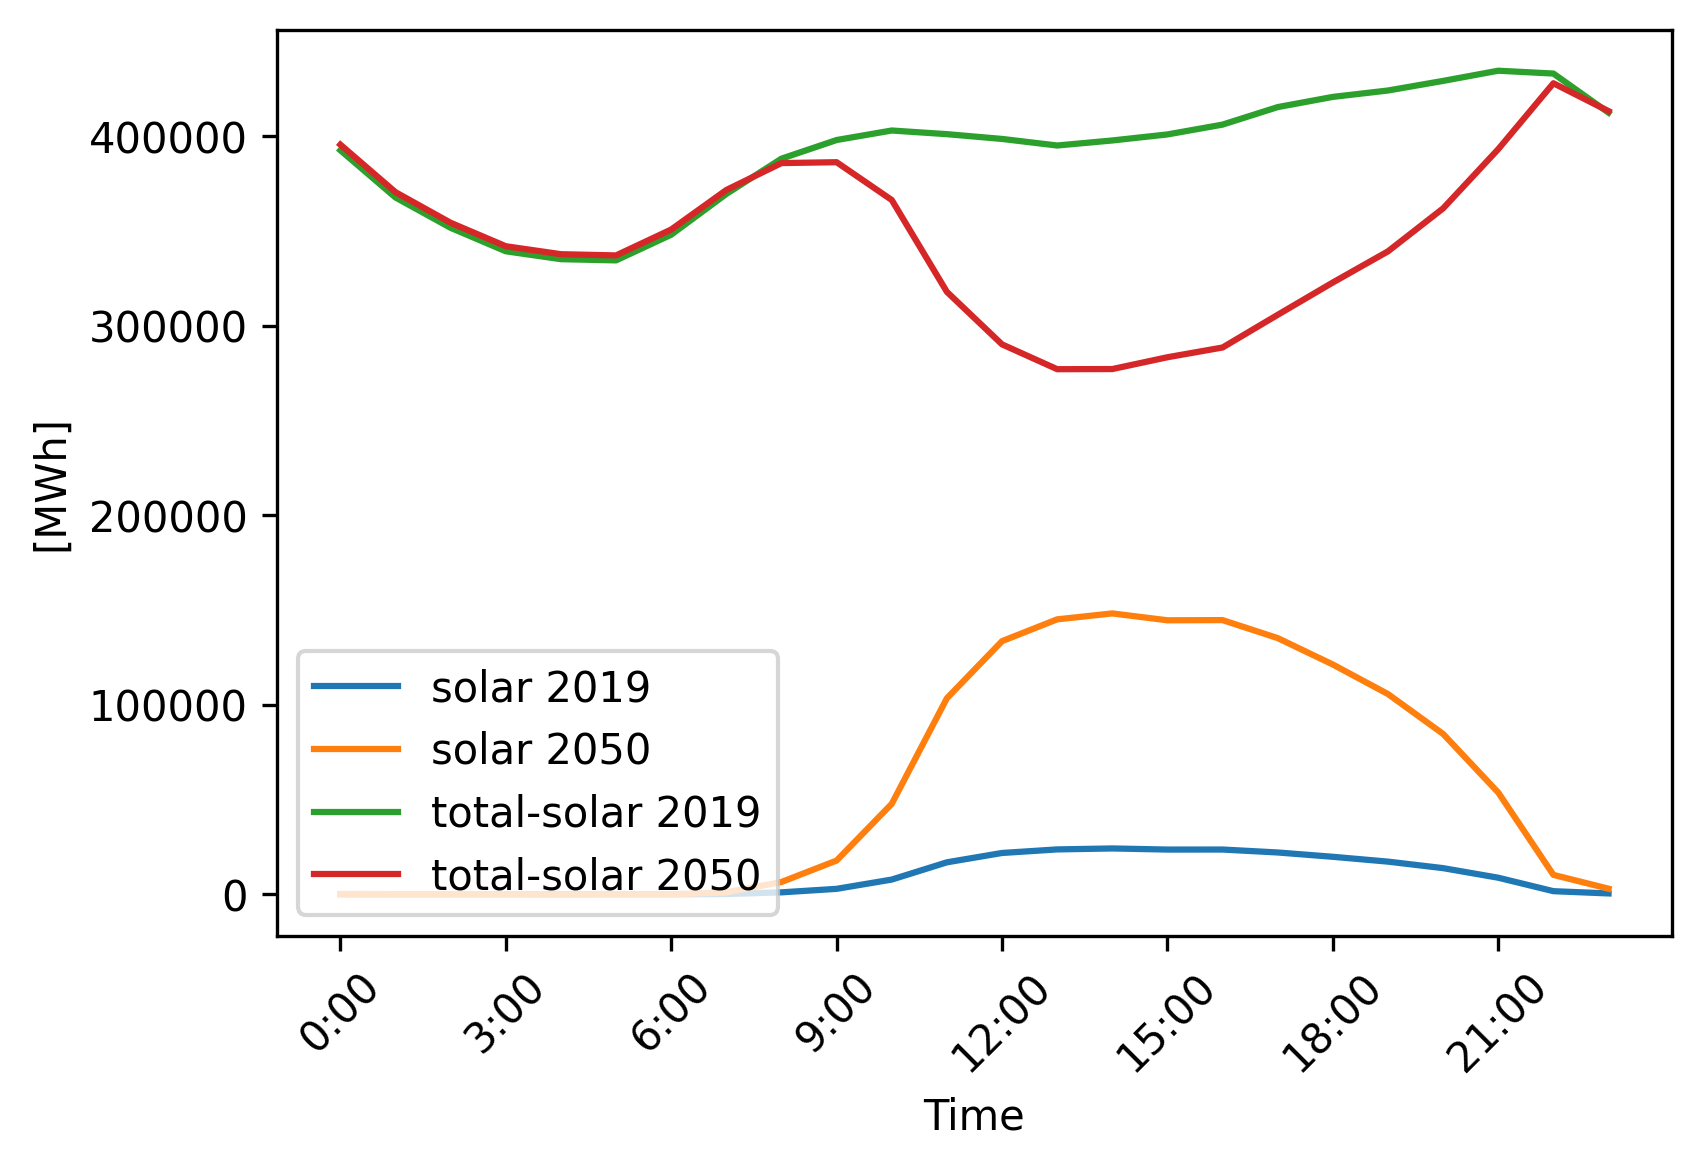
\includegraphics[width=1.0\linewidth]{figures/duck-curve4.png}
	\hfill
	\caption{Prediction on US demand for 2050.}
	\label{fig:us-duck}
\end{figure}

\begin{figure}[htbp!]
	\centering
	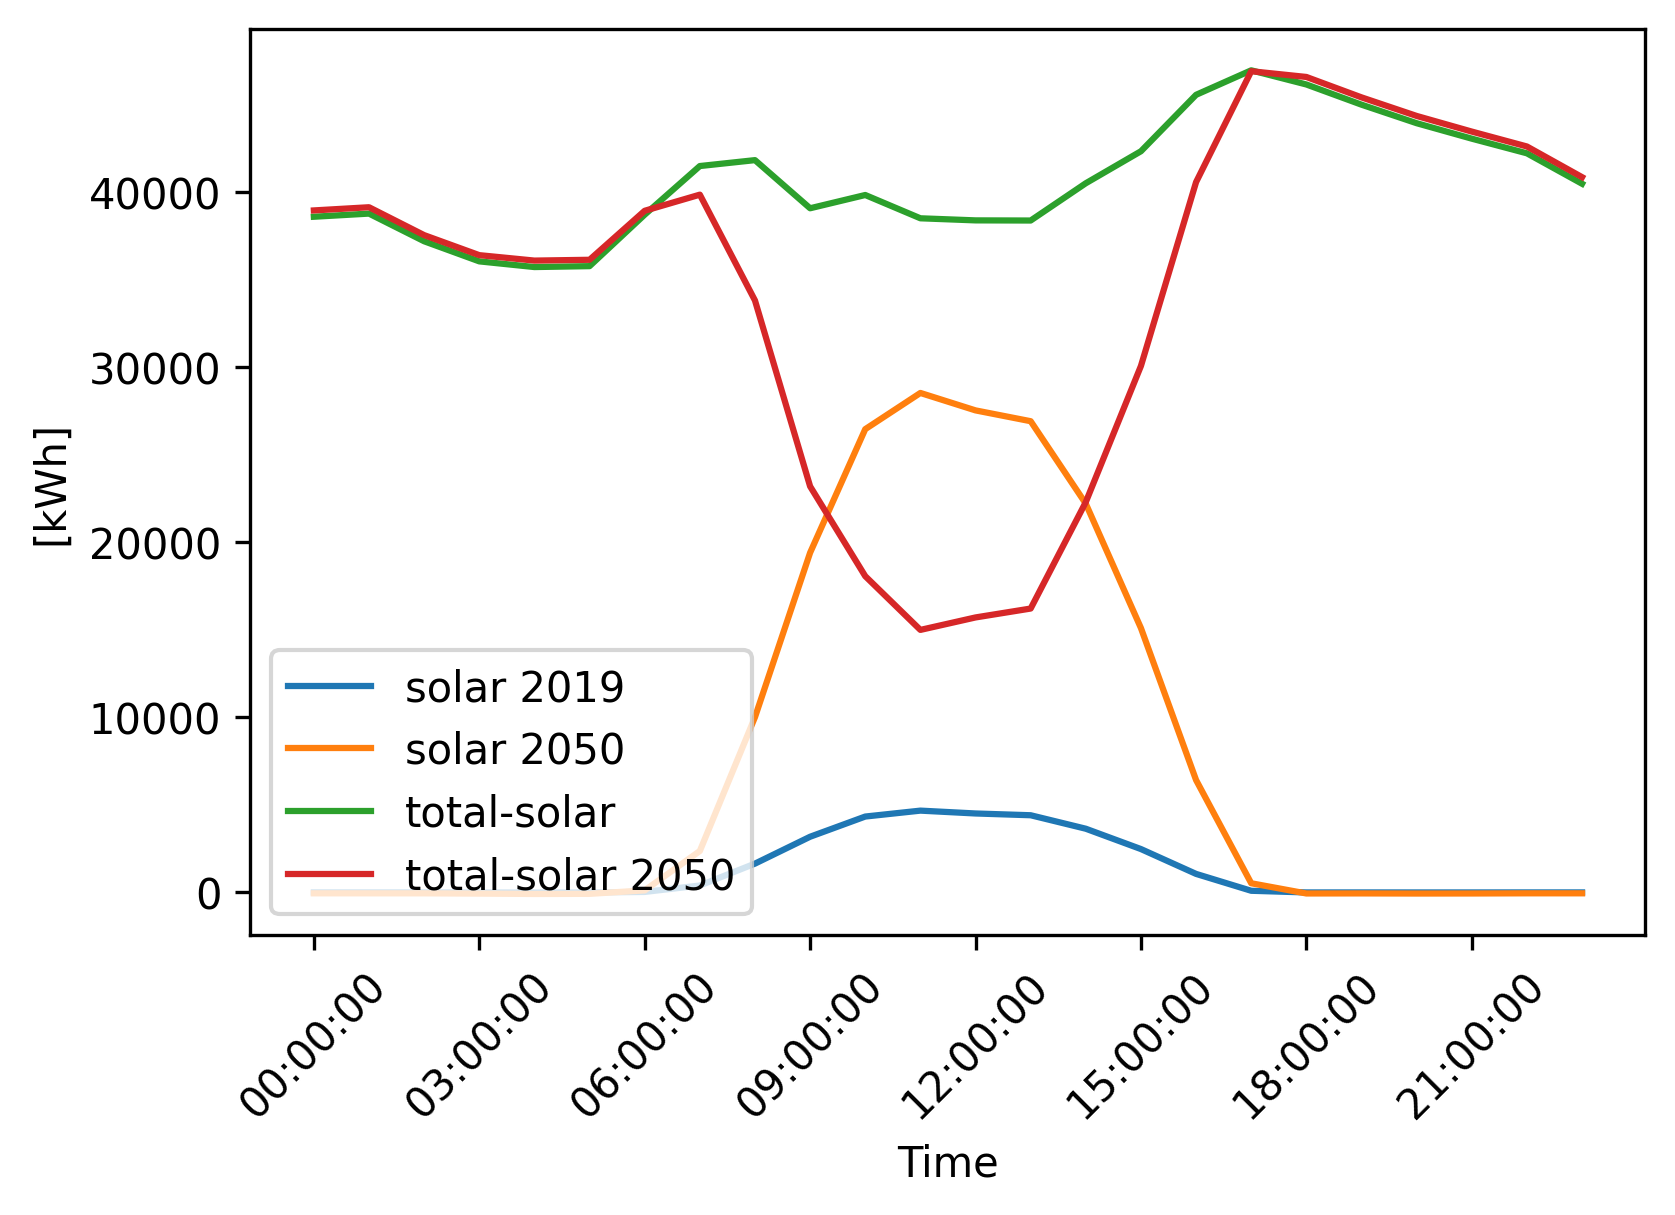
\includegraphics[width=1.0\linewidth]{figures/uiuc-duck.png}
	\hfill
	\caption{Prediction on UIUC's demand for 2050.}
	\label{fig:uiuc-duck}
\end{figure}

For the hydrogen production calculations, we chose a reactor of 25 MW.
Figure \ref{fig:uiuc-hydro2} displays the nuclear electricity generated by hour and the mass of hydrogen produced during the solar peak by \gls{LTE} and \gls{HTE}.
For the \gls{LTE} case, any type of reactor is a valid option.
The $\eta$ considered is of 33$\%$.
This yields a reactor power of 75.8 MW$_{th}$.
The H$_2$ production rate reaches a peak of 167 kg at 11 A.M.
During the day, the plant produces a total of 660 kg.
For the \gls{HTE} case, we chose an \gls{HTGR} with outlet temperature of 850$^{\circ}$C.
The $\eta$ considered is 49.8$\%$.
This yields a reactor power of 50.2 MW$_{th}$.
The H$_2$ production rate reaches a peak of 286 kg at 11 A.M.
During the day, the plant produces a total of 1136 kg.
Table \ref{tab:hydro} summarizes these results.

\begin{figure}[htbp!]
	\centering
	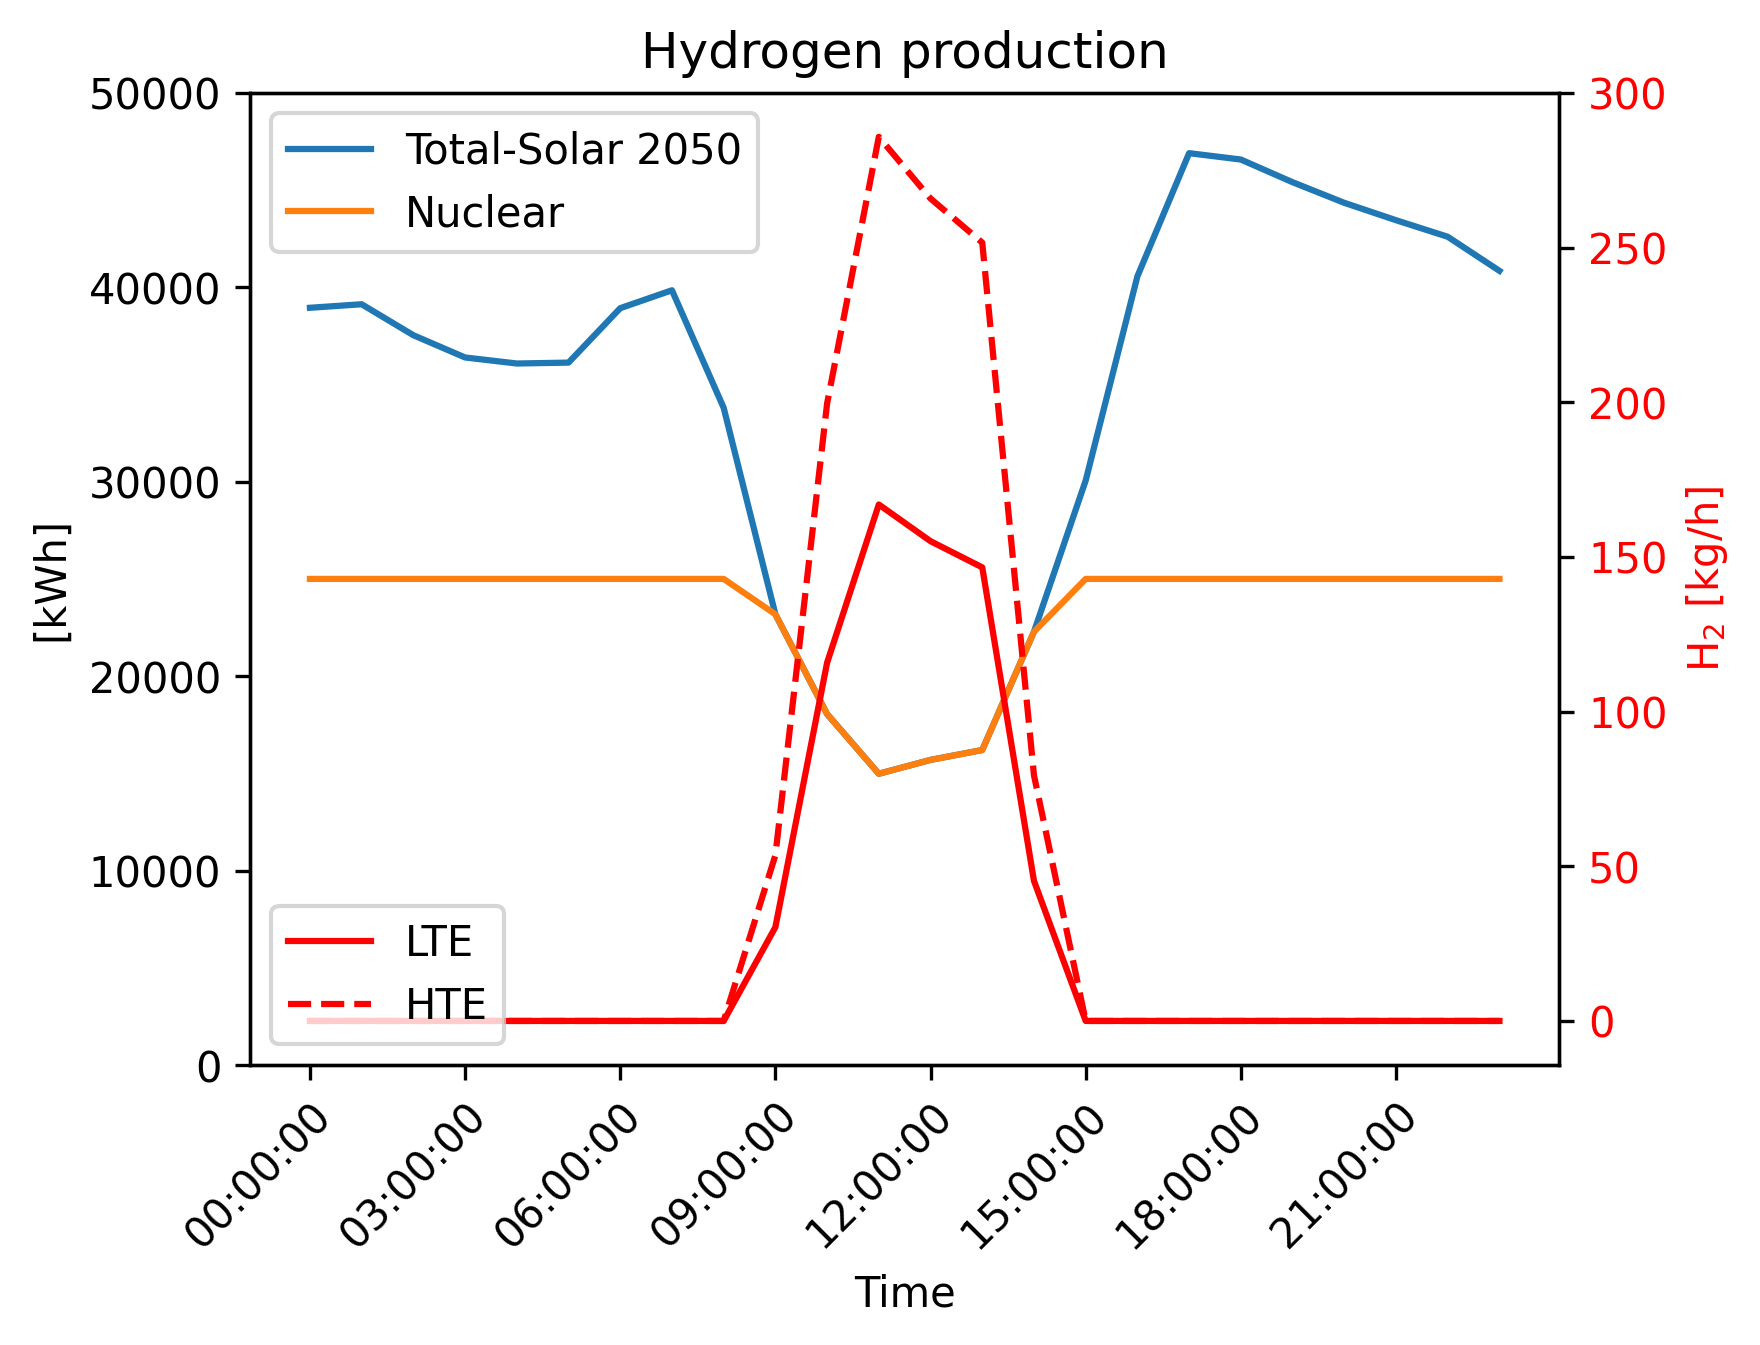
\includegraphics[width=1.0\linewidth]{figures/uiuc-hydro2.png}
	\hfill
	\caption{Hydrogen production with the excess of energy.}
	\label{fig:uiuc-hydro2}
\end{figure}

\floatsetup[table]{capposition=top}
\begin{table}[htbp!]
    \begin{tabular}{|lll|}
        \hline
        Process &  $\eta$ &  H$_2$ [kg]  \\ \hline
        \gls{LTE} &  33$\%$  &  660  \\ 
        \gls{HTE} &  49.8$\%$  &  1136  \\ \hline
    \end{tabular}
    \caption{Hydrogen production with \gls{LTE} and \gls{HTE}.}
    \label{tab:hydro}
\end{table}

% Word on these results.
The hydrogen produced with \gls{LTE} and \gls{HTE} generates 15843 and 27262 kWh, respectively. We use the hydrogen during the demand peak, between 4 PM and 10 PM. The new peaks are 41.89 MWh and 39.99 MWh.
Table \ref{tab:elect} summarizes these results. $DP$ is the difference between the old and the new peak.

\begin{figure}[htbp!]
	\centering
	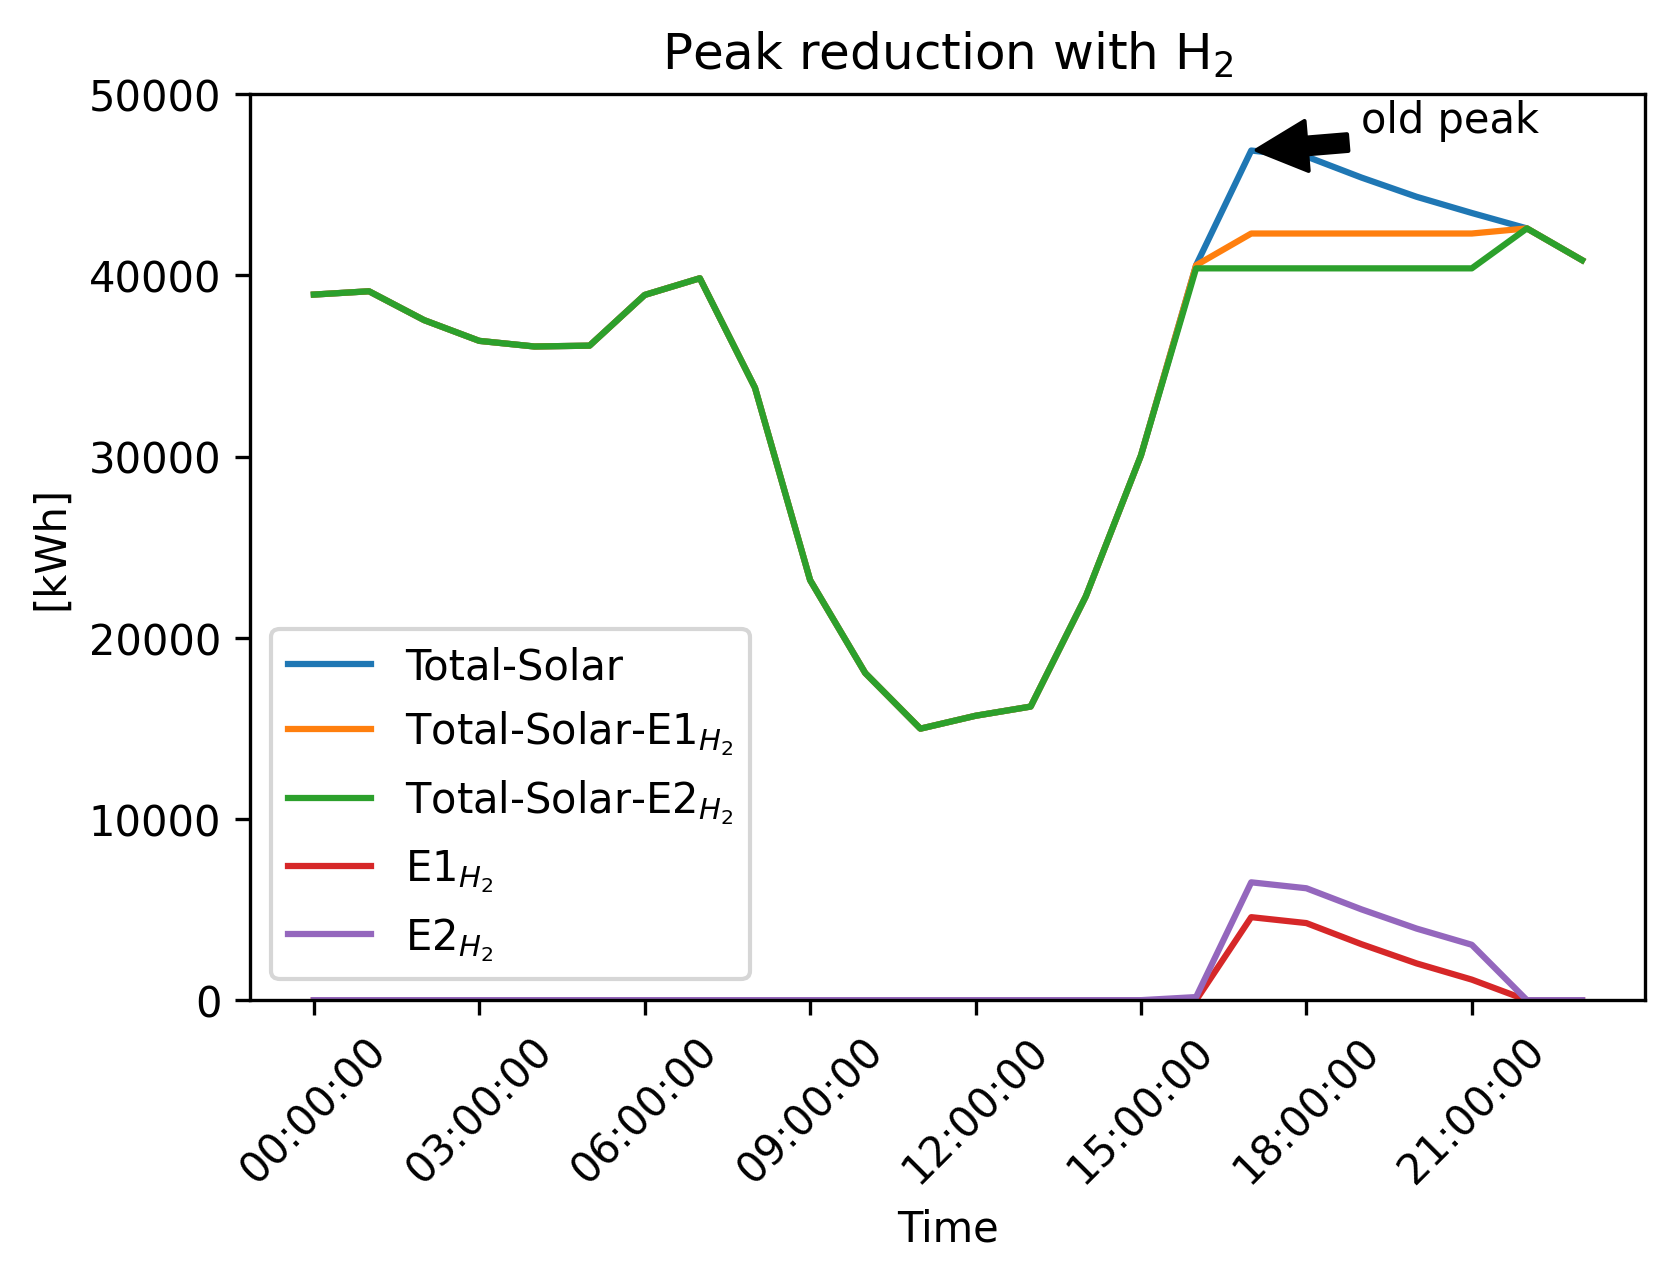
\includegraphics[width=1.0\linewidth]{figures/uiuc-hydro3.png}
	\hfill
	\caption{Peak reduction by using the produced H$_2$.}
	\label{fig:uiuc-hydro3}
\end{figure}

\floatsetup[table]{capposition=top}
\begin{table}[htbp!]
    \begin{tabular}{|llll|}
        \hline
        Process & E [kWh] & $NP$ [MWh] & $DP$ [MWh] \\ \hline
        \gls{LTE} & 15843 & 41.89 & 5.0 \\
        \gls{HTE} & 27262 & 39.99 & 6.9 \\ \hline
    \end{tabular}
    \caption{Electricity production with hydrogen produced with \gls{LTE} and \gls{HTE}.}
    \label{tab:elect}
\end{table}

\section{Conclusion and Future Work}

The analyzed data suggests that the duck curve phenomenon is likely to happen in the upcoming years.
Further studies could include more accurate predictions of both total and solar generation.
In the first case studied, the data takes the duck curve shape.
The demand ramp up that occurs in the evening does not look extremely alarming as it extends over a period of nine hours.
However, such ramp requires the grid to count with a high installed capacity of dispatchable sources.
On the other hand, this study underestimates the time over which the ramp occurs, as the data presented here integrates the whole country demand.
As the country is very wide and has several time zones, the peak demand occurs at different times for different regions. The same happens to the solar peak.
Further studies should carry out the same analysis but distinguishing the different regions.

Regarding \gls{UIUC} case, the results suggest that an excessive integration of \gls{PV} to the grid could be counter-productive.
The deployment of solar aligns with the carbon reduction objectives, but such deployment would require a high installed capacity of dispatchable sources to meet the demand.

Nuclear energy and hydrogen production proposes an approach to mitigate the negative implications of the duck curve.
While this article considers only two hydrogen production methods, there are a few more that could be coupled to a nuclear reactor.
Other studies could include those methods as well.
Furthermore, hydrogen introduces a way to store energy that would reduce the need of dispatchable sources to meet the demand.
Future work will examine the effects of deploying reactors of different sizes coupled to different hydrogen production methods.

One of the assumptions in the calculations is that when the demand is lower than the reactor power output, the reactor meets all the demand on its own.
That assumption is not realistic, as there are more non-dispatchable sources, as wind, integrated to the grid.
The assumption causes our study to underestimate the mass of hydrogen that could be produced, as the excess of thermal energy produced by the reactor would be higher.

%%%%%%%%%%%%%%%%%%%%%%%%%%%%%%%%%%%%%%%%%%%%%%%%%%%%%%%%%%%%%%%%%%%%%%%%%%%%%%%%
\bibliographystyle{ans}
\bibliography{bibliography}
\end{document}
